% This is "sig-alternate.tex" V2.1 April 2013
% This file should be compiled with V2.5 of "sig-alternate.cls" May 2012
%
% This example file demonstrates the use of the 'sig-alternate.cls'
% V2.5 LaTeX2e document class file. It is for those submitting
% articles to ACM Conference Proceedings WHO DO NOT WISH TO
% STRICTLY ADHERE TO THE SIGS (PUBS-BOARD-ENDORSED) STYLE.
% The 'sig-alternate.cls' file will produce a similar-looking,
% albeit, 'tighter' paper resulting in, invariably, fewer pages.
%
% ----------------------------------------------------------------------------------------------------------------
% This .tex file (and associated .cls V2.5) produces:
%       1) The Permission Statement
%       2) The Conference (location) Info information
%       3) The Copyright Line with ACM data
%       4) NO page numbers
%
% as against the acm_proc_article-sp.cls file which
% DOES NOT produce 1) thru' 3) above.
%
% Using 'sig-alternate.cls' you have control, however, from within
% the source .tex file, over both the CopyrightYear
% (defaulted to 200X) and the ACM Copyright Data
% (defaulted to X-XXXXX-XX-X/XX/XX).
% e.g.
% \CopyrightYear{2007} will cause 2007 to appear in the copyright line.
% \crdata{0-12345-67-8/90/12} will cause 0-12345-67-8/90/12 to appear in the copyright line.
%
% ---------------------------------------------------------------------------------------------------------------
% This .tex source is an example which *does* use
% the .bib file (from which the .bbl file % is produced).
% REMEMBER HOWEVER: After having produced the .bbl file,
% and prior to final submission, you *NEED* to 'insert'
% your .bbl file into your source .tex file so as to provide
% ONE 'self-contained' source file.
%
% ================= IF YOU HAVE QUESTIONS =======================
% Questions regarding the SIGS styles, SIGS policies and
% procedures, Conferences etc. should be sent to
% Adrienne Griscti (griscti@acm.org)
%
% Technical questions _only_ to
% Gerald Murray (murray@hq.acm.org)
% ===============================================================
%
% For tracking purposes - this is V2.0 - May 2012

\documentclass{sig-alternate-05-2015}


\begin{document}

% Copyright
\setcopyright{acmcopyright}
%\setcopyright{acmlicensed}
%\setcopyright{rightsretained}
%\setcopyright{usgov}
%\setcopyright{usgovmixed}
%\setcopyright{cagov}
%\setcopyright{cagovmixed}


% DOI
\doi{0}

% ISBN
\isbn{0}

%Conference
\conferenceinfo{FSS '16}{Aug 15--Dec 15, 2016, Raleigh, NC, USA}

\acmPrice{0}

%
% --- Author Metadata here ---
%\conferenceinfo{WOODSTOCK}{'97 El Paso, Texas USA}
%\CopyrightYear{2007} % Allows default copyright year (20XX) to be over-ridden - IF NEED BE.
%\crdata{0-12345-67-8/90/01}  % Allows default copyright data (0-89791-88-6/97/05) to be over-ridden - IF NEED BE.
% --- End of Author Metadata ---
\title{A Review On Random Forest In Biological And Medical Data}
%\subtitle{Random Forest and .....}

\numberofauthors{2}
\author{
% 1st. author
\alignauthor
Michael Herzog\\
       \affaddr{Department of Computer Science}\\
       \affaddr{North Carolina State University}\\
       \affaddr{Raleigh, North Carolina}\\
       \email{mherzog@ncsu.edu}
% 2nd. author
\alignauthor
Sandeep Reddy Katypally\\
       \affaddr{Department of Computer Science}\\
       \affaddr{North Carolina State University}\\
       \affaddr{Raleigh, North Carolina}\\
       \email{skatypa@ncsu.edu}
}

\maketitle
\begin{abstract}
This paper reviews Random Forest. Therefore we start with a paper of 2008 that uses Random Forest and review papers for each year up to 2016. New approaches and comparison are described and critically scrutinized. Extensions that has been added to the Random Forest framework are also described and compared to each other. All paper's content is the analysis of medial or biological data. Those date has certain differences to other datasets. The differences and their effects are described and the usage of Random Forest on those datasets is evaluated.
\end{abstract}


%
% The code below should be generated by the tool at
% http://dl.acm.org/ccs.cfm
% Please copy and paste the code instead of the example below. 
%
\begin{CCSXML}
<ccs2012>
<concept>
<concept_id>10010147.10010257.10010321</concept_id>
<concept_desc>Computing methodologies~Machine learning algorithms</concept_desc>
<concept_significance>500</concept_significance>
</concept>
%todo
</ccs2012>  
\end{CCSXML}


\ccsdesc[500]{Random Forest~Machine learning algorithms}
%todo


%
% End generated code
%

%
%  Use this command to print the description
%
\printccsdesc

% We no longer use \terms command
%\terms{Theory}

\keywords{Random Forest, Curse of dimensionality, Medical Data, Biological Data}

\section{Introduction}
The course of dimensionality is a well-known problem in the field of medical and biological data science. Due to the large amount of features, it is very complicated to extract the features or combination of features with the most influence on the class labels. Medical or biological data normally consists of many rows and few columns. This paper reviews the development and the variants of a machine learning algorithm called Random Forest. Starting from the 2012 paper by Touw et al. "Data mining in the Life Sciences with Random Forest: a walk in the park or lost in the jungle?" \cite{touw2012data} we take a look back and forwards with focus on the applied methods. We show how Random Forest and its variants perform in the biological or medical context.

Random Forest \cite{breiman2001random} is a machine learning method for classification and regression. The motto of random forests is, ``If one tree is good, why not build a whole bunch?'' \cite{Robillard:recomm_sys_sw_eng}. An ensemble of trees is used to detect the most popular class.

Schwarz et al. \cite{schwarz2010safari} propose Random Jungle, a software package, which is based on Random Forest. It was said to be up to 159 times faster than alternative approaches. One reason for that is the implemented so called ``variable backward'' elimination. The variable backward elimination drops features as long as they aren't enough significant. The significance level is set manually prior.  Random Jungle also allows a parallel computation of trees, which is very suitable for datasets with a large number of features. So many trees can be grown in parallel. As mentioned by Touw et al. in their paper it was the fastest Random Forest implementation. 

Willows \cite{zhang2009willows} is a software package that uses Random Forest as well as a classification tree and a deterministic forest. It's purpose is to maximize the computer memory and to allow an analysis of massive genotype data, which is a particular type of biological data. 

Hapfelmeier and Ulm \cite{hapfelmeier2013new} developed a new way for variable selection and tested it against eight other approaches for variable selection. Random Forest has been shown to perform well for high prediction accurancy and distinguishing between important and unimportant variables. Their new way, they say, distinguishes even better than the other approaches between important and unimportant variables while it is still as fast as the others. Their baseline idea is to use permutation to produce unbiased importance measures.

In Maken et al. \cite{maken2014multiple} Random Forest is compared to kNN and the multiple instance learning method (MIL). Their subject is a biomedical topic. They use the methods for the classification of Breast Cancer using Magnetic Resonance Imaging. They use generic (tile-biased) as well as domain specific features (region-of-interest). The subject of detecting breast cancer is a more graphical use of classification, in which Random Forest also performs well.
``Data mining and linked open data - New perspectives for data analysis in environmental research'' \cite{lausch2015data} provides an overview on techniques that can be used. Their idea behind is to give an overview of existing data mining techniques due to the increase of the amount of data that is collected in the 22th century. They also confirm the use of Random Forest in the topics Medicine and Biology, which are of type spatial data mining, image mining or text mining. All in all the paper shows mainly the different tools which can be used for the analysis of big data in different fields of interest.

The 2016 paper ``On the use of Harrel's C for clinical risk prediction via random survival forests'' \cite{Schmid2016450} uses the Harrel's C as a split criterion for the so called Random Survival Forest. ``Random Survival Forest'' \cite{ishwaran2008random} extends the Random Forest towards survival data. Normally Random Survival Forest use the log-rank split criterion. The new approach, Harrel's C, is compared to the common criterion in the 2016 paper. They come to the conclusion to use Harrel's C in smaller scale clinical studies and the log-rank split criterion for use in large-scale `omics' studies.

The following sections TODO


\section{Motivation}
Biological and medical data are of specific kind. They usually have a lot of features and and often few samples, compared to the number of features. This kind of data also have features that interact strongly with each other. The improving technology lets researchers collect much data that has to be analyzed. The stepping up in sequencing DNA for example reveals a lot of genetic code. The complexity of genetic diseases can be simplified by using classification models. Or the images that are obtained by imaging method like Magnetic Resonance Imaging have to be classified. The large amount of data is also to be considered for the use of computational memory and calculation power.

Random Forest is a framework that is said to perfom well on this specific kind of data. It is especially known for its high precision accuracy. As said Random Forest is a framework. The motivation of this paper is to show how Random Forest is used and implemented for the specific kind of data. Different approaches and extensions are shown in this paper.

\section{Hypothesis}
The hypothesis in the paper we studied were all about a faster implementation or a implementation that classifies their specific kind of data better than other approaches. A faster implemention is said to be done by a better use of the computer memory or a better parallelization. All in all the hypothesis is that Random Forest performs well on biological and medical data. It is said to have a high precision accurancy and that it can extract interactions between features well.

\section{Background}
Data that comes from medical and biological resarches is special, because it often consists of very many features compared to their samplesize. Random Forest is said to perform well on these kind of data. We first give an introduction to the data with its specialities and then fundamental overview on how Random Forest works.

\subsection{Medical and Biological Data}
Research in Biological topics, especially in gene-gene, protein-protein or Genome-wide interactions as well as Biological Sequence analysis or medical topics like cancer detection lead to high-dimensional data. The improving methods to collect data in those topics result in a data explosion, which makes the use of machine-learning techniques popular. Extracting meaningful information of high-dimensional data is a challenging task. That also affects the computation time, and the convergence towards a solution. The decreasing ability of algorithms to converge by the increasing size of dimensions is called ``The curse of dimensionality''.
The term  describes the fast increasing of a volumina while adding more dimensions. Data sets in life science normally have a lot more variables than samples. Figure \ref{fig:curse_dim} illustrated the curse of dimensionality. On the left side you see a two dimensional table. The blue square indicates the volume by using 2 dimensions and both only the range from zero to one. The volume already increases 16 times when using a range of zero to four. The volume even more increasis by adding additional dimensions as shown by the cube in the right side. Using the range zero to three for all three dimensions increases the volume of the  little blue cube 27 times.

\begin{figure}
\centering
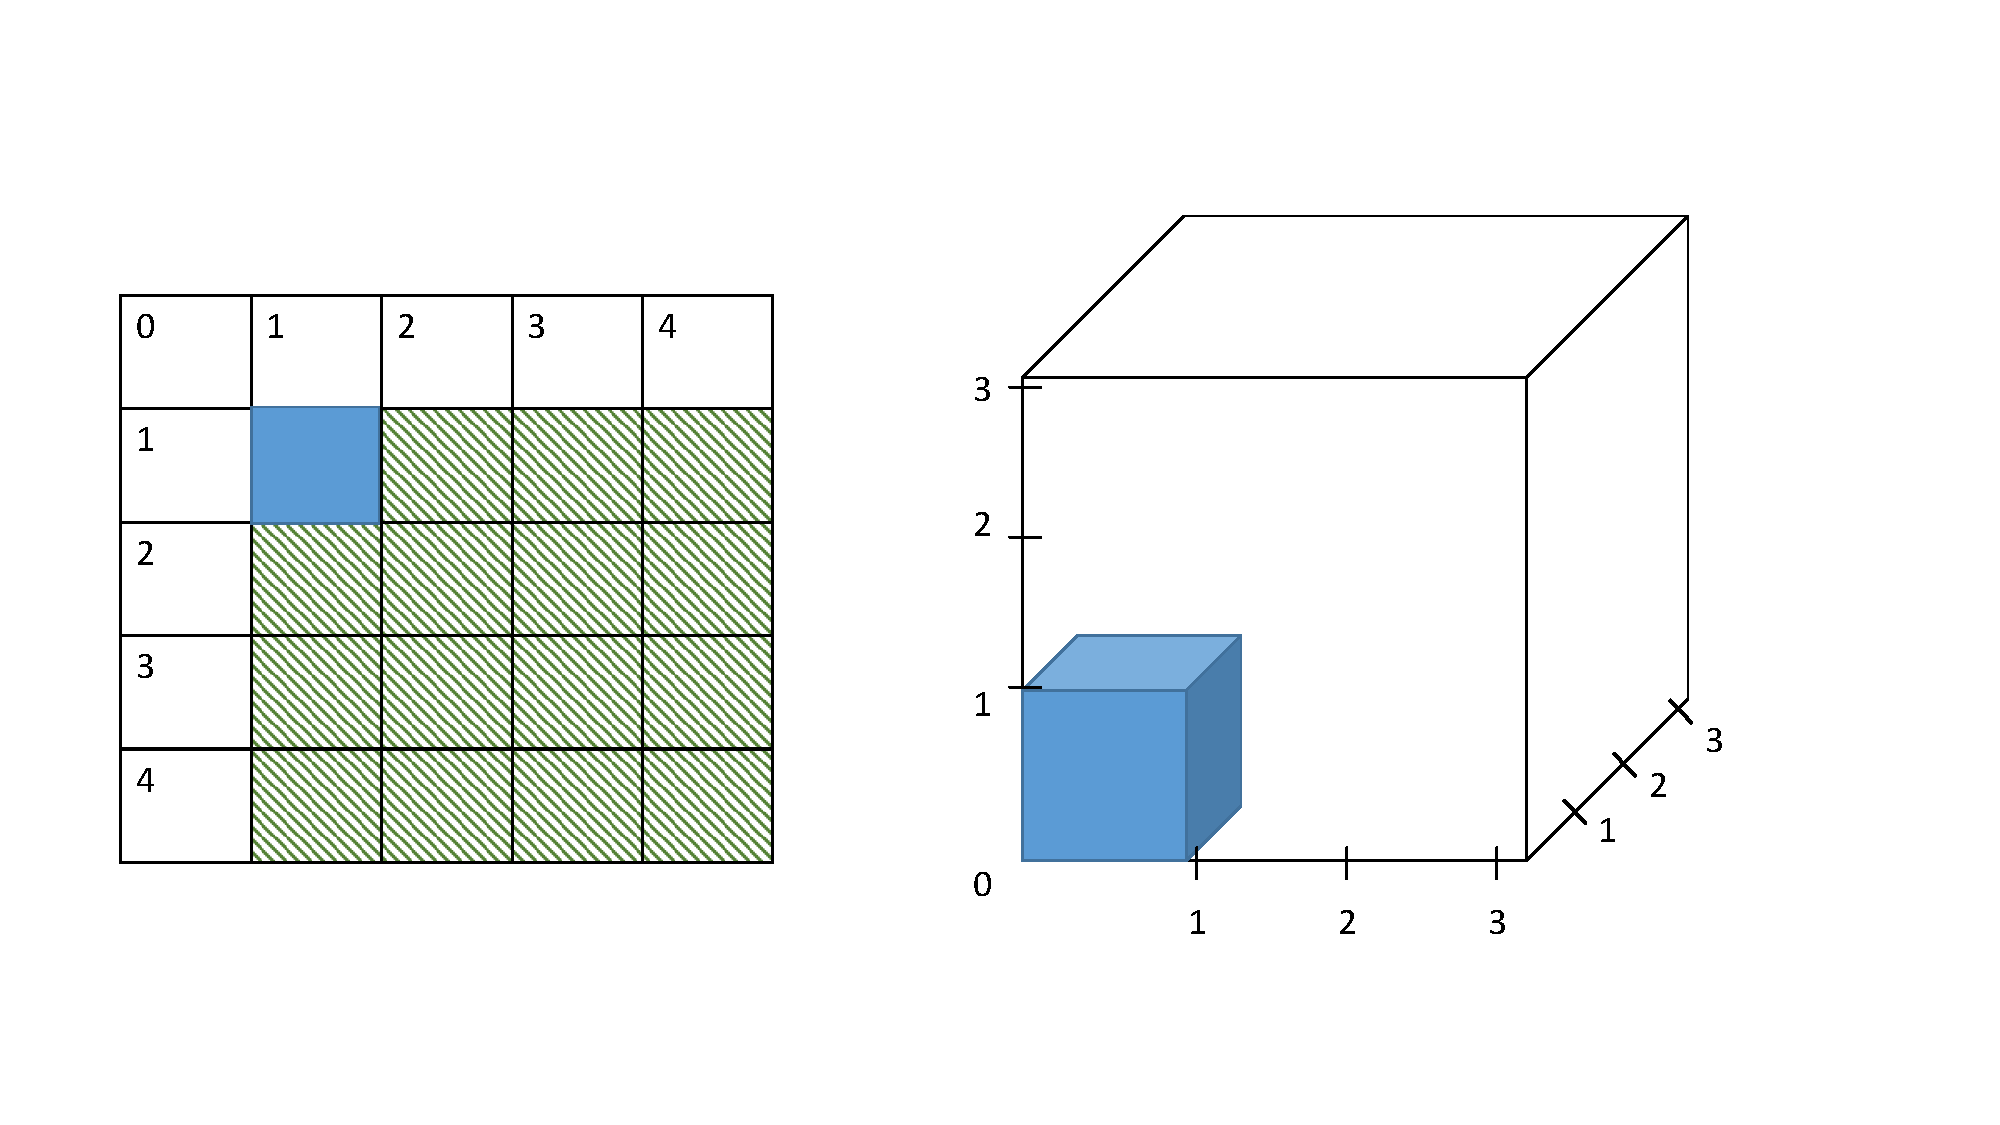
\includegraphics[width=3.5in]{curse_dim}
\caption{Illustration of the curse of dimensionality}
\label{fig:curse_dim}
\end{figure}

Often in biological and medical science the sampling size is small. This in combination with many dimensions makes a computation difficult, because using so many features would require a large amount of training data. The Hughes phenomenon addresses that problem: The predictive power reduces as the dimensionality increases, using always the same number of training samples \cite{1054102}.
But those two are not the only issues that one has to deal with. Another phenomenom is called ``confound of multimodality'' \cite{clarke2008properties}. This term refers to the complexity of biological systems. In biological data we often have to handle multiple interrelated biological processes, which blurs the relationship between two genes for example. Whenever needed, that problem is described specifically in this paper.
At last there is also a strong correlation between the features. Iinteractions between variables can cause an effect, respectively variables can sometimes become important when they interact with other variable.

\subsection{Random Forest}
The Random Forest is very suitable to use in medical or biological data. It has not only a good prediction accurancy but also a very good interpretability compared to other machine learning algorithms \cite{qi2012random}. Random Forest is also very fast, since it can be used concurrently.

The trees are built like follows until every feature was used.
\begin{itemize}
\item Randomly select $d$ samples with replacement
\item $ \sqrt{n}$ out of $n$ features are selected for one tree.
\item The features are evaluated for their ability to split the data, the one with the best ability is selected to split the set into subdatasets.
\item Recursivley repeat the feature selection on the subdatasets until every leave is prune or the leaves contain a certain number of samples.
\end{itemize}
Random Forest is thus an ensemble method, the name comes from the randomly selected samples and features. Notice that the trees are not pruned afterwards.  After all trees are built, the training phase is completed.

In the test phase a test sample is predicted by every tree in the forest. The final decision for the class label of the test sample goes by the majority of predicted classes.

Note that only one tree without the other of the forest is not a good decision tree, because it only handles a subset of features. But when all trees in the forest are used, you get a strong qualifier \cite{touw2012data}. In addition there is no need for a cross-validation, because every tree already contains training and test data.

\begin{figure}
\centering
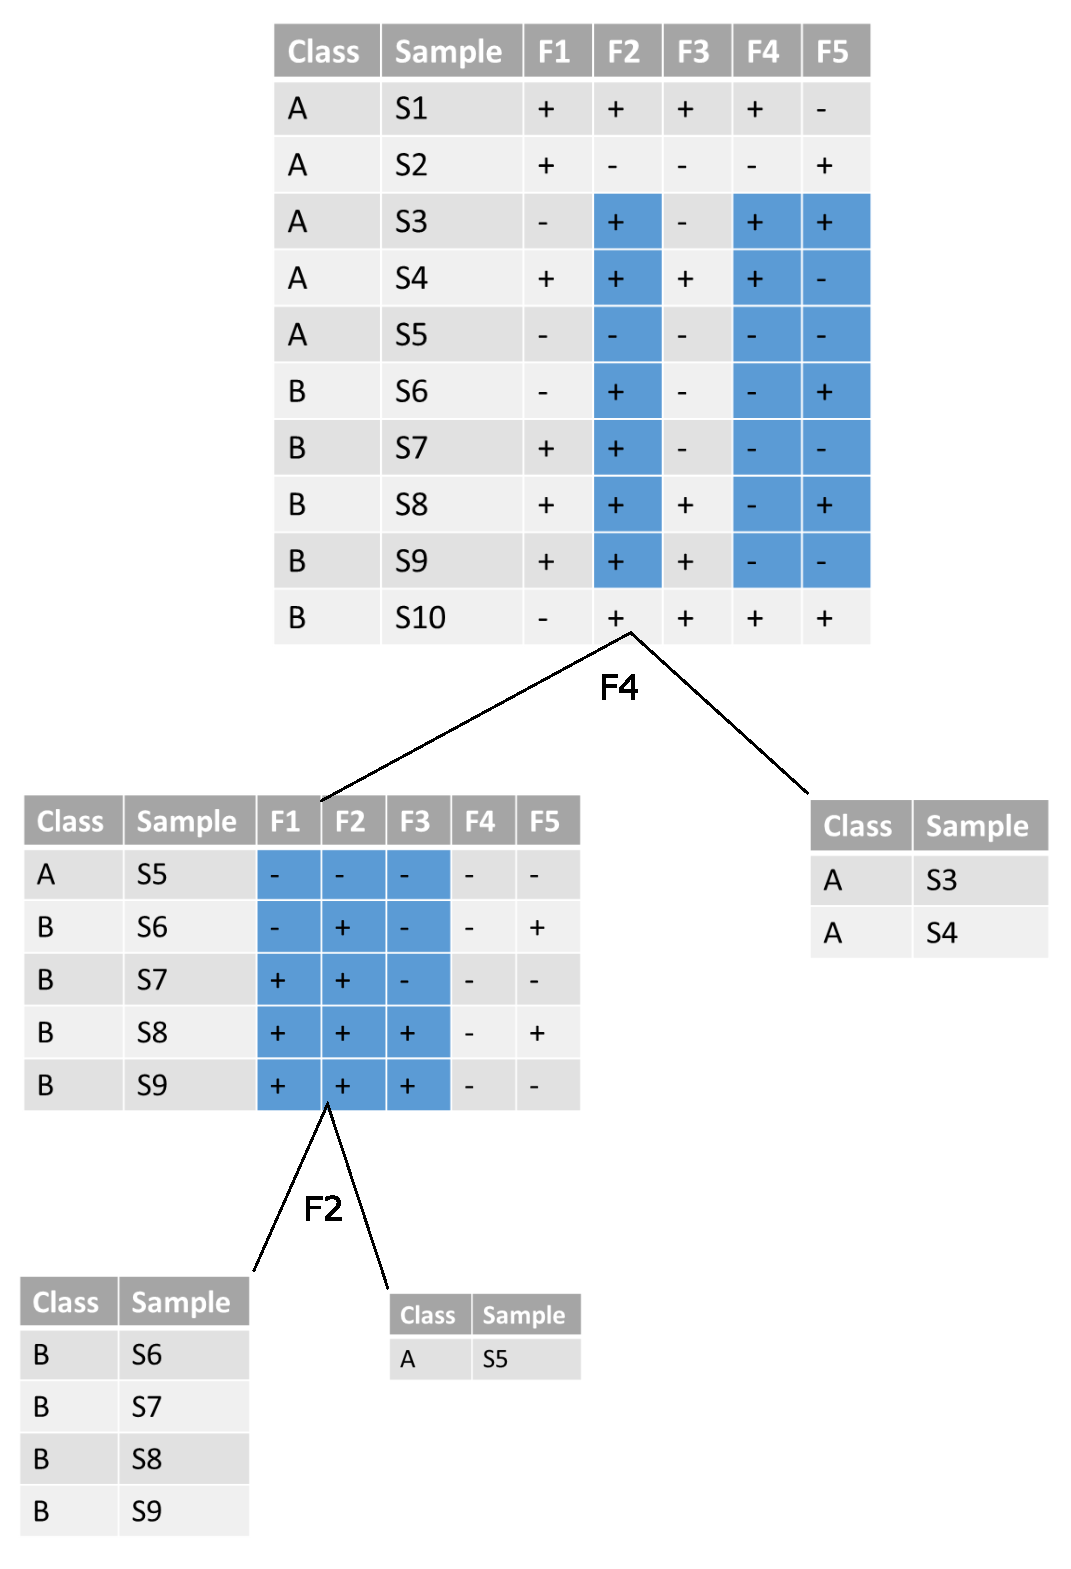
\includegraphics[width=3.5in]{rf}
\caption{Building of one tree of the forest by Random Forest}
\label{fig:rf}
\end{figure}

Figure \ref{fig:rf} illustrates the building of one tree of the forest. On top F2, F4 and F5 are the randomly selected features and S3-S9 are the randomly selected samples. The randomly selected area is painted blue. F4 splits the data best, so there is a leave on the right branch containing only samples that are of class A. The left side of the branch is the rest, it is still mixed up, so we again select randomly features, here F1-F3. F2 does the best split, which results in two leaves, the one on the left side containing only samples that are of class B and on the right branch a sample of class A. Now that all leaves are not mixed up at all, the algorithm determins. Now other trees have to be built in the same way until we obtain a forest.

\section{Checklists}
All datasets are roughly similar structured. They all use data from biological or medical research. Some are open available and used on certain workshops like the Genetic Analysis Workshop 15. Some paper, however don't mention the origin of their dataset. In the paper about Multiple Instance Learning for Breast Cancer they split their data into only mass-like and both mass-like and non-mass-like lesions. Willows describes in his paper that he uses a binary representation of his samples, they only have four different outcomes, so they can be represented by two bits. Other datasets aren't specifically prepared for the analysis.

Checklists are to prevent mistakes because of forgetting things. So for data science with the medical and biological context we should always know which the used algorithm is for and if it is not exactly appropriate, we should adapt it. We should keep in mind that it is complex data and therefore we need enough time to interpret the results. Due that the amount of data is large we should make safe that the environment we run our analysis on is computationally able to handle the data.

\section{Study instruments}
In all the papers the don't use study instruments like surveys. The data collected in medicine \cite{nmd2004szolo}, though, normally contains a lot of data about the patient which can only be gained by asking him or letting him fill out a sheet. Features in medical data are for example
\begin{itemize}
\item Family history
\item Patient's medical history
\item Medication
\item Current complaint
\end{itemize}
as well as data gained from measurements or recorded signals (EKG, EEG,...). Medical, as well as biological data, contain data like genom data which can not be obtained by surveys. They are measured by a medical or biological procedure.

\section{Statistical Tests}
A statistical test provides a mechanism for making quantitative decisions to determine whether there is enough evidence to ``reject'' a null hypothesis. Most of the papers were about a faster performance, so it suggests itself to perform a comparison of performance.
So for example in the paper ``On safari to Random Jungle'', they plot their results in addition which makes the result even noticeable. Figure \ref{fig:onsafaribar} shows their bar chart.

\begin{figure}
\centering
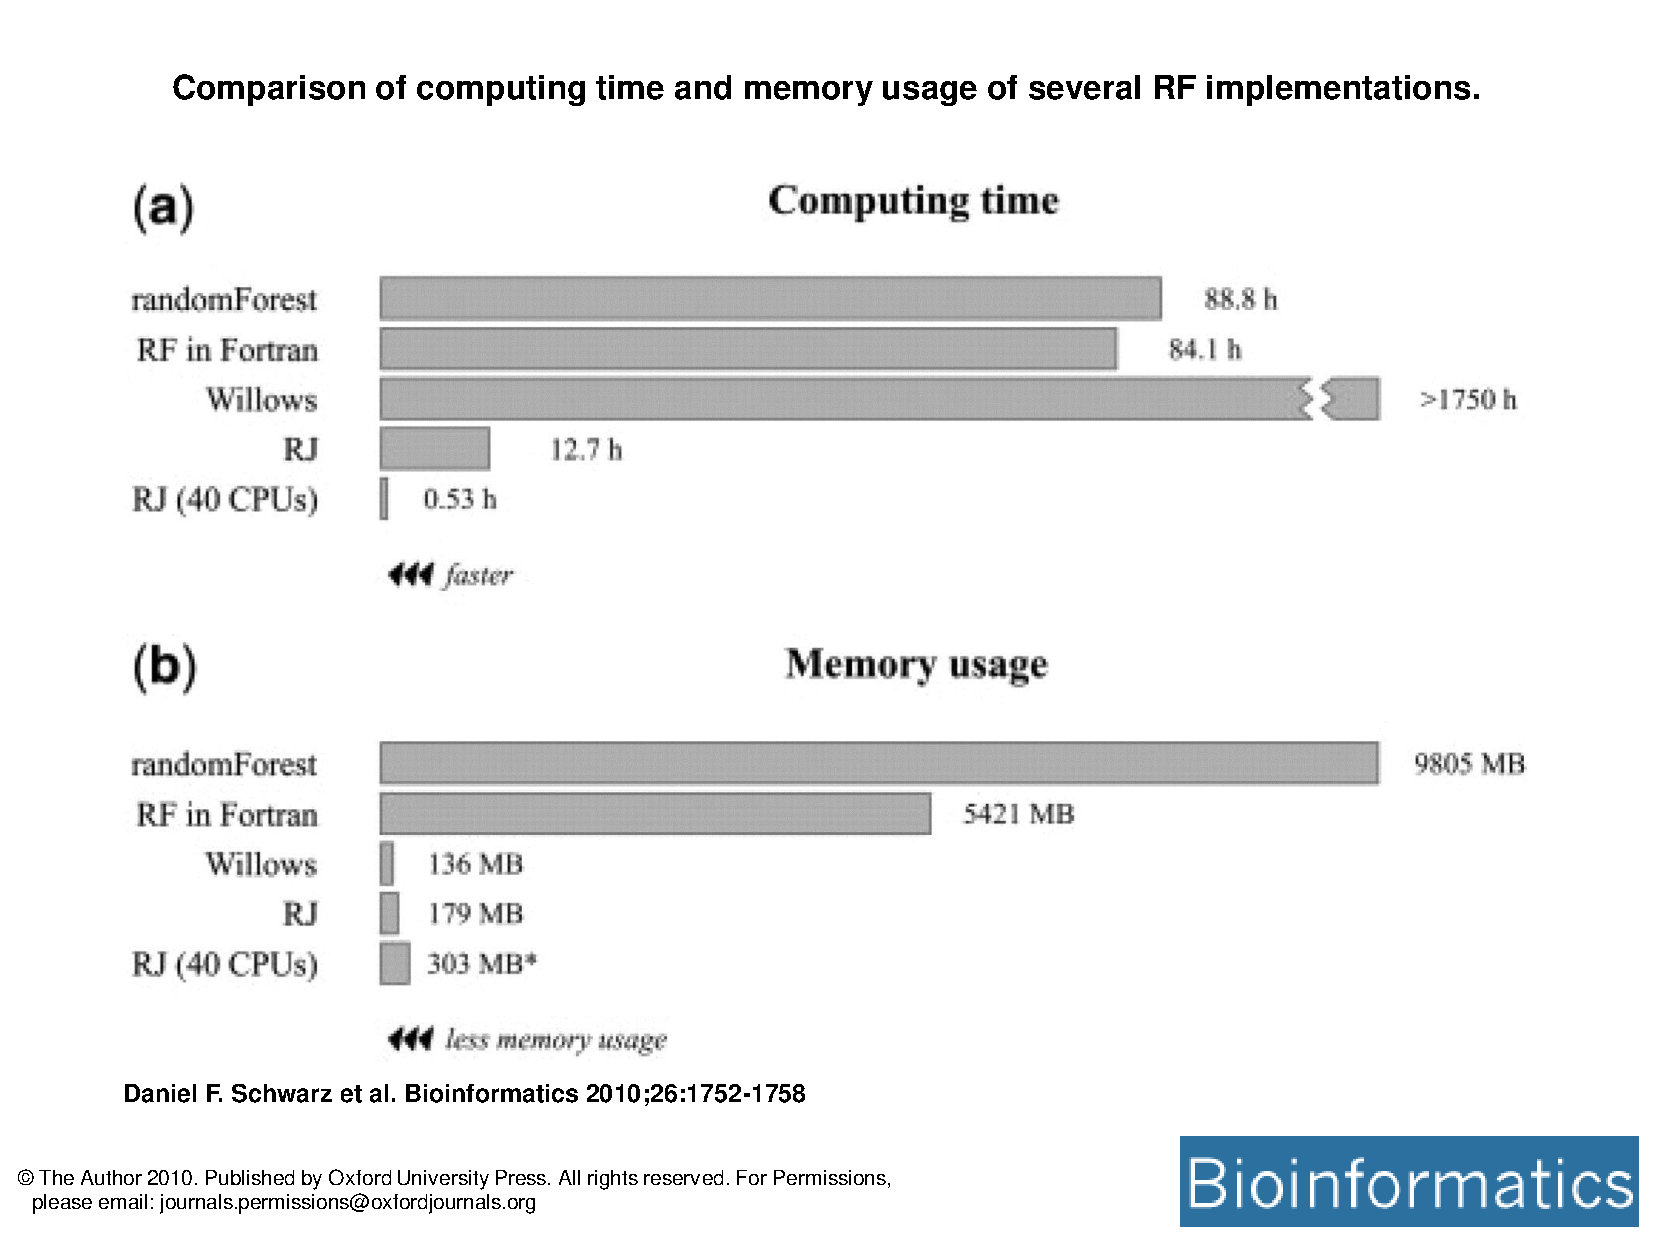
\includegraphics[width=3.5in]{onsafaribar}
\caption{Comparison of computing time and memory usage, in \cite{schwarz2010safari}}
\label{fig:onsafaribar}
\end{figure}

Zhang, Wang and Chen illustrate their performance results in a table. Figure \ref{fig:willowstable} shows their table used to compare run time.

\begin{figure*}
\centering
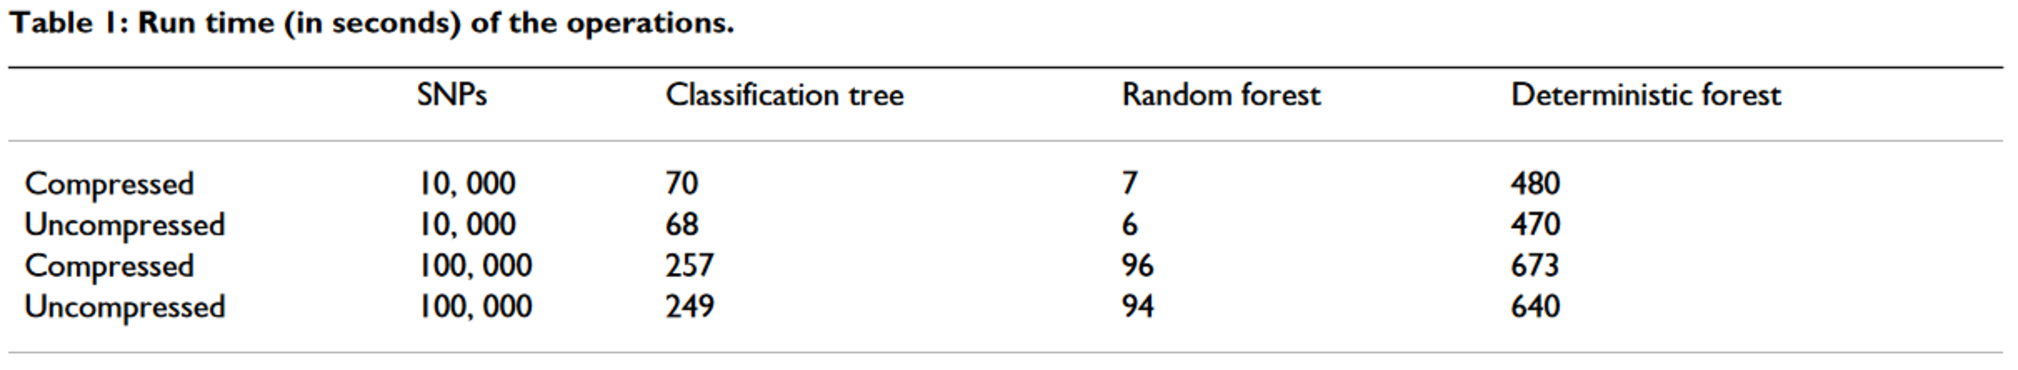
\includegraphics[width=5in]{willowstable}
\caption{Comparison of run time \cite{zhang2009willows} }
\label{fig:willowstable}
\end{figure*}

In ``On the use of Harrell's C for clinical risk prediciton via random survival forest'' Schmid, Wright and Ziegler use Boxplots of performance differences between to methods in log scale as can be seen in Figure \ref{fig:harrellscbox}.

\begin{figure*}
\centering
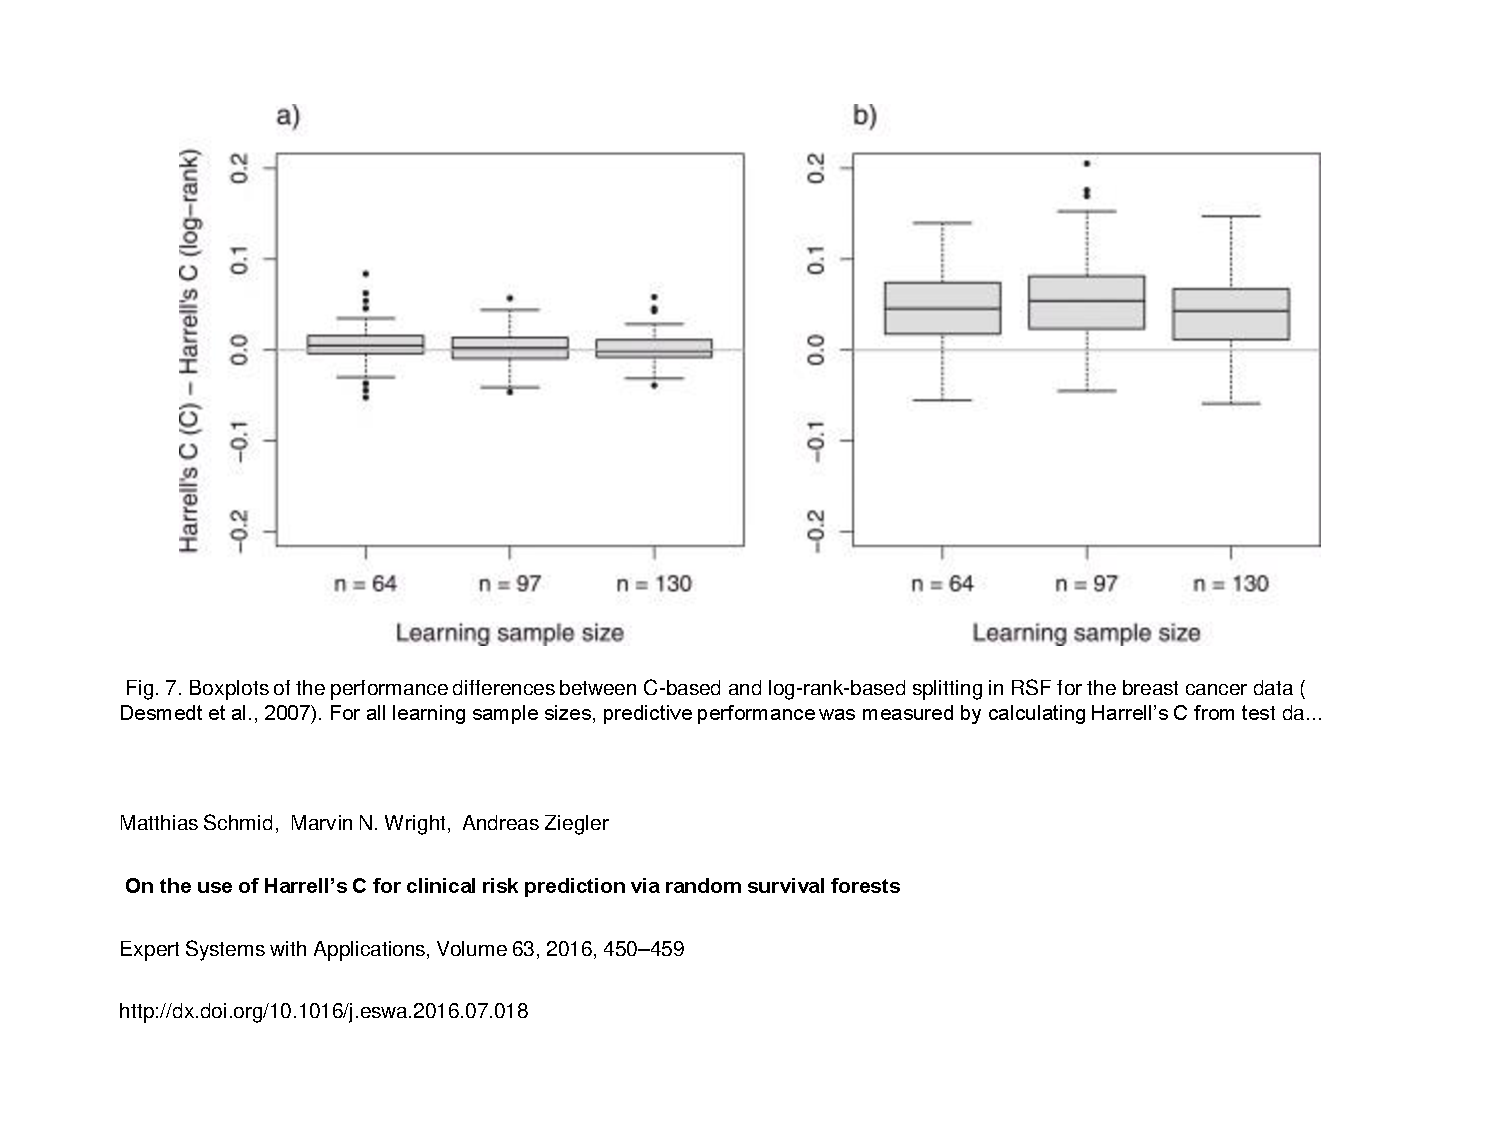
\includegraphics[width=5in]{harrellscbox}
\caption{Comparison performance using boxplots in \cite{Schmid2016450}}
\label{fig:harrellscbox}
\end{figure*}

In \cite{schwarz2010safari} they also introduce the proximity between samples. Those are measurements of the similarity of samples. So, outliers can also be predicted by the proximity measurements. The identification of those or of mislabeled samples can be seen as a feedback and can let the researcher take a deeper look on them.

Touw et al. compared a lot of sutdies and they got to say that 66\% of the studies use the ``variable importance''. Consider a large dataset with a lot of features. Variables that are very important for a subset can be lost when only looking at the global result. So the local variable importance can be though very important for the classification of a sample.

Zhang, Wang and Chen \cite{zhang2009willows} compare values that are received across several repetition of their performed permutation to reflect the empirical distribution of importance measures and to obtain $p-values$. In addition they also use the so called ``Test-Wise Error Rate (TWER)'' which can be seen as the probability that the null-hypothesis is rejected, but should not be subjected and the ``Family-Wise Error Rate (FWER)'' which is used in multiple hypothesis testing and is the probability of getting at least one false positive test.

Bradley et al \cite{maken2014multiple} use the Mean area under receiver operating characteristics curve (AUC) as the performance measurement. They also compare two AUCs arising from different algorithms using a t-test. A t-test tests the significance of a difference between two sets.

\section{Baseline results}
The oldest paper we examined is ``FACIL: fast and accurate genetic code inference and logo'' \cite{dutilh2011facil}. FACIL was implemented due to a new sequencing method for DNA, which resulted in new and large datasets. Random Trees with standard parameter was used to assess the correctness of their homology-based predicitons. That increased the precision and sensitivity scores. 
As said, in the oldes paper they used the standard parameter. In the next two papers \cite{schwarz2010safari} and \cite{zhang2009willows} the Random Forest is tuned to perfom better.
Random Jungle is said to perform up to 159 times faster than alternative implementations while still produce valid results. Figure \ref{fig:onsafaribar} illustrate their results. The upper image shows that Random Jungle both running on one processor or 40 performs way faster than the other implementations. Random Jungle in an extension to Random Forest which can be run on multiple processors. Random Jungle can perform Random Forests on multiple processors. For that it uses multithreading and Message Passing Interface parallelization. Random Jungle also uses the ``variable backward elimination''. Their results for the importance scores shows equal performance compared to Random Forest.

Regarding the lower part of Figure \ref{fig:onsafaribar} shows the memory usage.
Here Willows performs best, the parallelization by Random Jungle costs a little more memory due to the parallelization demands. Willows also was implemented to run on a normal desktop computer, the authors also used a 2.33 GHz processor and 2 GB physical memory running on Microsoft Windows XP Professional Version. Willows use the recursive partitioning technique: A classification rule predicts membership and consists of a predictor and its corresponding threshold. After the splitting rule is applied on the first root, the daughter roots are split and afterwards their daughter rules - recursively.

Figure \ref{fig:willowstable} shows the performance of Random Forest in comparison to Classification tree and Deterministic Forest. Having 10 000 SNPs, Random Forest performs 10 times faster than Classification tree and 68-78 times faster than Determenistic Forest. With 100 000 SNPs the performance of Random Forest was also better than Classification tree (2.6--5 times) and approcimately 7 times faster than Deterministic Forest.
The main ouput is tree structures as shown in figure \ref{fig:willowstree}

\begin{figure}
\centering
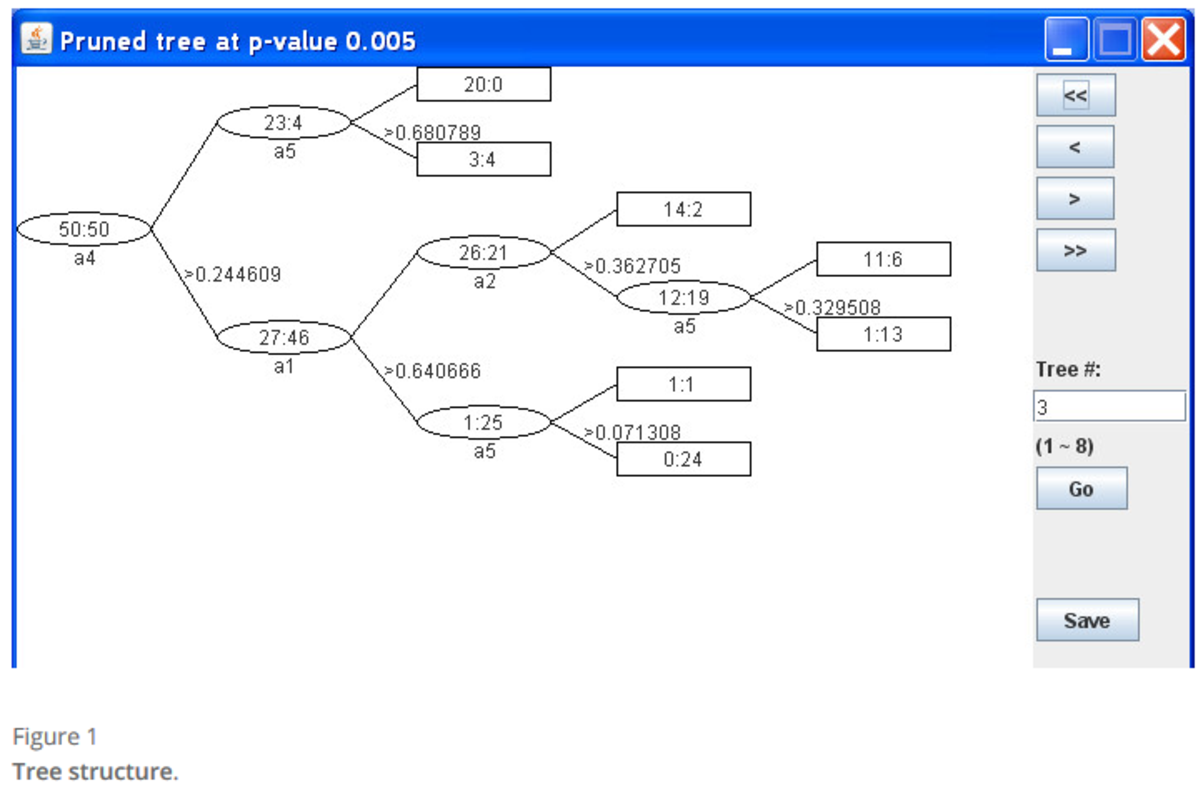
\includegraphics[width=3in]{willowstree}
\caption{Sample resulting tree, \cite{zhang2009willows}}
\label{fig:willowstree}
\end{figure}

The next paper ``A new variable selection approach using Random Forest'' \cite{hapfelmeier2013new} is beat-off in this series of different Random Forest implementations and extensions. This paper is about a new approach to select variables. Selection variables on a higher point of view is the process of selecting a subset of relevant features (variables, predictors) for use in model construction. They did an extensive review on variable selection methods and came to the conclusion that they wanted to develop a new one. Their new approach is based on the theoretical framework of permutation tests and meets important statistical properties, and can be applied to regression and classification problems. They took four famous datasets so that they are accessible to everyone who wants to reproduce the results in the future. They selected four data sets, two regression datasets and two classification datasets. They datasets were chosen such that they had differing number of variables and observations. At the end they came to the conclusion that to prove generalizability, the benefit of its application, concerning prediction accuracy and especially the selection of relevant variables, has to be further investigated. Further investigations need to be done to explore factors like correlation strength, block size, interactions, type of importance measure, definition of `relevance' and kind of alpha adjustment which were identified to affect variable selection. 

The authors of the 2014  paper ``Multiple instance learning for breast cancer magnetic resonance imaging'' \cite{maken2014multiple} compare Random Forest against citation-kNN and tile-kNN, and investigate how Multiple Instance Learning performs in comparison. For that they use utilise both tile-based  and region-of-interest  (ROI)  based features. 

For the tile-based features  a subimage is seen taken like one bag of feature vector, which are extracted from one individual tile. Due to the size, classification performance is not affected by the accuracy of the segmented regions. A region-of-interest  (ROI)  based feature is a part of samples that have been specially selected due to a specifc purpose. In this paper, based on the data each lesion becomes a labelled instance in the dataset. The features extracted from each lesion are then individually labelled as either benign (negative) or malignant (positive)  \cite{maken2014multiple}. 

The results show that citation-kNN works better than tile-based kNN. The performance of ckNN is the same as ROI-based SIL. They say ckNN is a suitable choice, in addition they figured out that it could be used as screening tool under certain circumstances. But apparently, the best mean AUC which is there measurement is obtained with Random Forest. The better classification performance of Random Forest comes from the robustness of Random Forest and its variable selection method. Figure \ref{fig:mildataa} shows that a difference  between  citation-kNN  and  tile-based  kNN is significant, while the  difference between citation-kNN  and  tile-based   single   instance   RF   is   not   statistically   significant.   All in all Random Forest performs best, but not significantly.

\begin{figure}
\centering
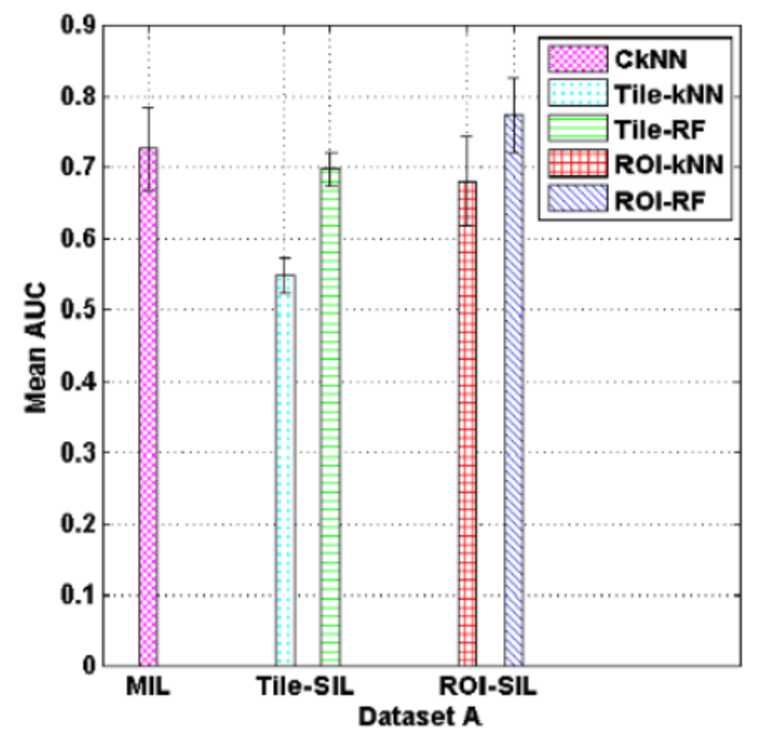
\includegraphics[width=3in]{mildataa}
\caption{Comparison of results, \cite{maken2014multiple}}
\label{fig:mildataa}
\end{figure}

The youngest paper in our series is ``On the use of Harrell's C for clinical risk prediction via random survival forests'' \cite{Schmid2016450}. Here Harrell's C is proposed as the split criterion. They perform their measurements on Random Survival Forest.
All in all they recognize that  Harrell's C perfomfs well as a split criterion for smaller studies, while the log-rank splitting better performs in lager-scale data. 

\section{Patterns, Negative Patterns, Negative Results}
In the FACIL paper the second step of the algorithm sometimes performs very bad. The homology-based prediction caused a very low precision (24\%) for stop codons. But unfortunately they don't even mention why they use the randomForest R package.

A ngeative result of Random Jungle occurs when running the Random Jungle software to perform random forests on a multi-core processor, it consumes more memory than when run on a single-core processor. This is because because helping data structures have to be provided for every core of the processor. They lack in addition in the explanation how Random Jungle technically works.

The use of Willows reduces the amount of needed memory but this decreases its speed. So an improvement of the memory usage  brings a negative effect on the performance. But in this paper there is less theoretical beckground explained, a implementation of their algorithm only out of the paper wouldn't work.

The paper about the a new variable selection approache lacks in where this method will not work should be explained. Furthermore why it will not work in certain situations could also be explained. 

Lausch et al's paper also shows the following antipattern: The discussion is very big. It could be more precise and they did not explain why they chose the data sets the chose. 

Only two paper compare their results to other methods than Random Forest. 

\section{New Results}
We recognized a lot of new results as well as the verification that Random Forest really works at least as good on medical and biological data as other classifiers. No other classifier could perform better than Random Forest. New result were the highly increased speed of Random Jungle, which is an extension to Random Forest and the more efficient usage of computer memory shown by Willows. A different approach for a variable selection could also not perform better than Random Forest. 


\section{Future Work}
The biological and medical data is very complex. Almost all methods need to be verified more that they were in the paper mentioned. The particular problem of those data is that the features correlate highly with eacht other. That means that an approach that splitting on one feature is sufficient is not accurate. A proper analyzation of medical and biological systems also needs a lot of samples, since there are so many features and it is affected by the course of dimensionality. In addition biological and medical creatures always have certain unique attributes. So that is also to be considered.



%\end{document}  % This is where a 'short' article might terminate

%ACKNOWLEDGMENTS are optional

%
% The following two commands are all you need in the
% initial runs of your .tex file to
% produce the bibliography for the citations in your paper.
\bibliographystyle{abbrv}
\bibliography{sigproc}  % sigproc.bib is the name of the Bibliography in this case
% You must have a proper ".bib" file
%  and remember to run:
% latex bibtex latex latex
% to resolve all references
%
% ACM needs 'a single self-contained file'!
%
%APPENDICES are optional
%\balancecolumns

%\balancecolumns % GM June 2007
% That's all folks!
\end{document}
